\documentclass[a4paper]{article}
\usepackage[margin=2cm]{geometry}

\def\pgfsysdriver{pgfsys-pdftex.def}

\usepackage{fontspec}
\usepackage[english]{babel} % Language 
\usepackage{enumitem}
\usepackage{listings}
\usepackage[dvipsnames]{xcolor}
\usepackage{graphicx}
\usepackage{float}
\usepackage[hidelinks]{hyperref}
\usepackage{tikz}
\usepackage{pgfplots}
\usepackage[dvipsnames]{xcolor}
\usepackage{multirow}
\usepackage{caption}
\usepackage{tabls}
\usepackage{pdfpages}

\setlength{\parindent}{0pt}
\setlength{\parskip}{1em}

\lstset{
	basicstyle=\ttfamily,
	showspaces=false,
	showstringspaces=false,
	tabsize=4,
	stringstyle=\color{orange},
	commentstyle=\color{OliveGreen},
	keywordstyle=\color{blue},
	numberstyle=\color{Gray},
	frame=single
}

\title{
	\textsc{PAR: Laboratory 3} \\
	\texttt{\large par4201}
}

\author{Joan Marcè i Igual \and Esteve Tarragó i Sanchís}


\begin{document}

\maketitle
\tableofcontents
\pagebreak

\section{Task granularity analysis}

\begin{enumerate}
	\item Which are the two most important common characteristics of the task graphs generated for the two task granularities (\textit{Row} and \textit{Point}) for the non-graphical version of \texttt{mandel-tareador}? Obtain the task graphs that are generated in both cases for \texttt{-w 8}.
\end{enumerate}

For the non-graphical version of \verb|mandel-tareador| the most important charactersitc is that both tasks are parallelizable while the graphical version is not parallelizable. 

\begin{figure}[H]
	\centering
	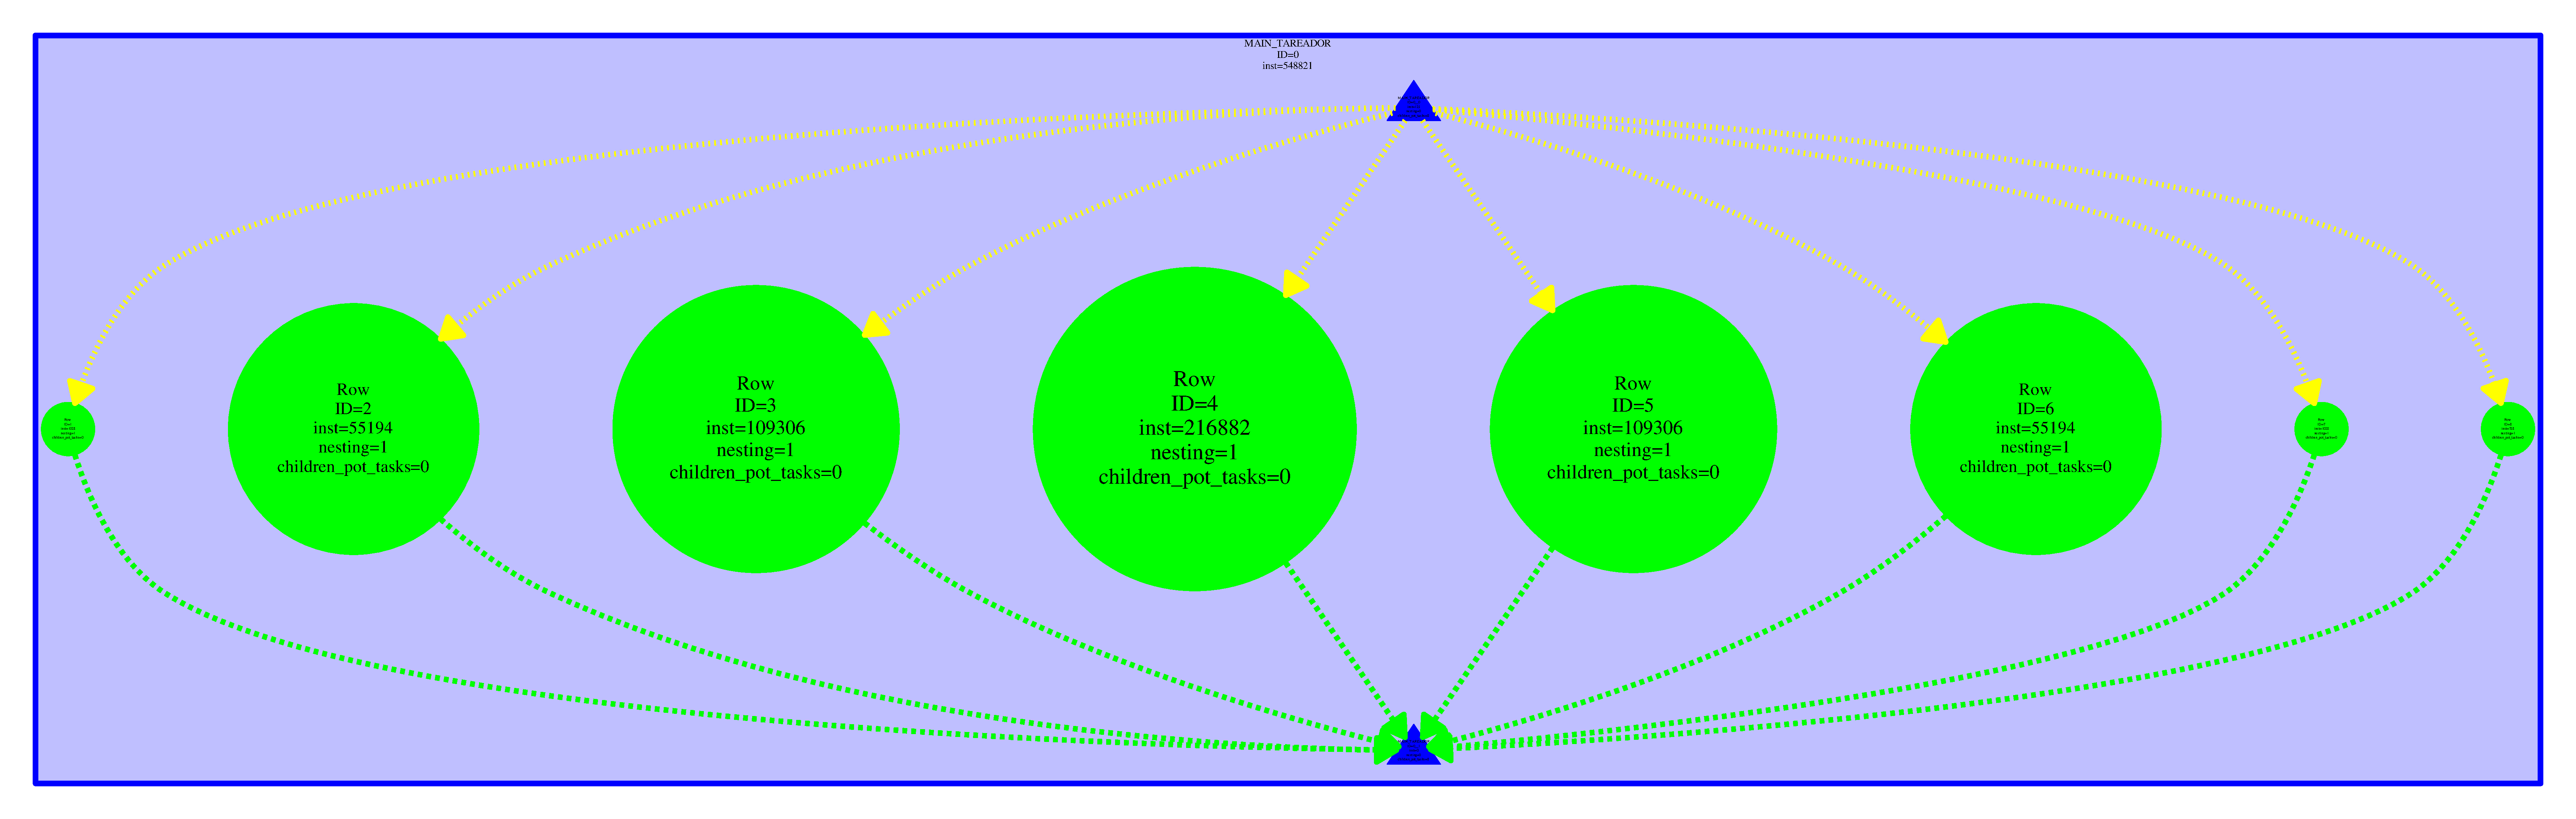
\includegraphics[width=\textwidth]{images/depend_row_text.pdf}
	\caption{Row based task parallelization generated by \texttt{Tareador}}
\end{figure}
\begin{figure}[H]
	\centering
	\includegraphics[width=\textwidth]{images/depend_point_text.pdf}
	\caption{Point based task parallelization generated by \texttt{Tareador}}
\end{figure}

\begin{enumerate}[resume]
	\item Which section of the code is causing the serialization of all tasks in \texttt{mandeld-tareador}? How do you plan to protect this section of code in the parallel OpenMP code?
\end{enumerate}

The section of the code that is causing the serialization of all tasks in the graphic version is the following:

\begin{lstlisting}[language=C]
 if (setup_return == EXIT_SUCCESS) {
  XSetForeground (display, gc, color);
  XDrawPoint (display, win, gc, col, row);
 }           
\end{lstlisting}

To protect this section of code I will make it a critical section of the code:

\begin{lstlisting}[language=C]
if (setup_return == EXIT_SUCCESS) {
#pragma omp critical
	{
		XSetForeground (display, gc, color);
		XDrawPoint (display, win, gc, col, row);
	}
}           
\end{lstlisting}

\section{\texttt{OpenMP task-}based parallelization}

\begin{enumerate}
	\item For the \textit{Row} and \textit{Point} decompositions of the non-graphical version, include the execution time and speed–up plots obtained in the strong scalability analysis (with \texttt{-i 10000}). Reason about the causes of good or bad performance in each case.
\end{enumerate}

\begin{figure}[H]
	\centering
	\begin{minipage}[b]{0.49\textwidth}
		\centering
		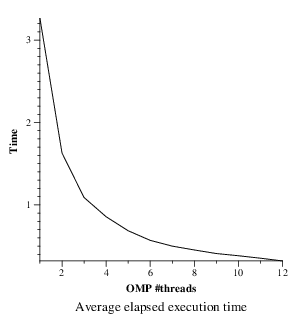
\includegraphics[width=\textwidth]{images/image10}
		\caption{Point speed-up}
	\end{minipage}
	\begin{minipage}[b]{0.49\textwidth}
		\centering
		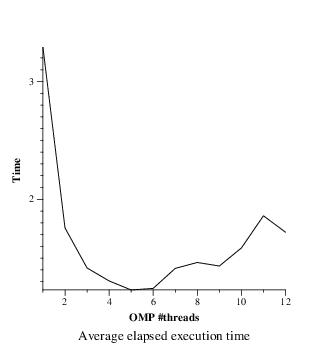
\includegraphics[width=\textwidth]{images/image00}
		\caption{Point time}
	\end{minipage}
\end{figure}
\begin{figure}[H]
	\centering
	\begin{minipage}[b]{0.49\textwidth}
		\centering
		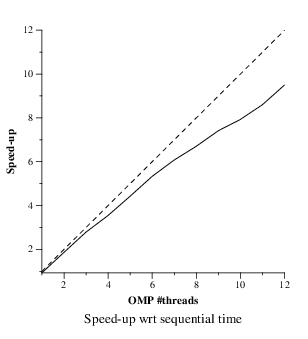
\includegraphics[width=\textwidth]{images/image11}
		\caption{Row speed-up}
	\end{minipage}
	\begin{minipage}[b]{0.49\textwidth}
		\centering
		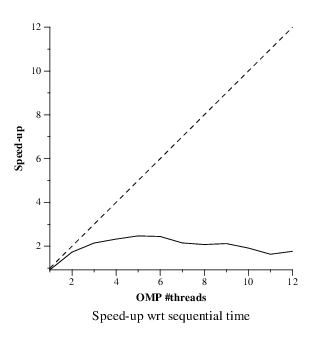
\includegraphics[width=\textwidth]{images/image01}
		\caption{Point speed-up}
	\end{minipage}
\end{figure}

In both cases we see that the overhead increases with the number of threads. When running the point version the overhead is so big that it performs better with 6 threads than with more. 


It’s much better to choose the granularity to row because there is an overhead that increases with the number of task to assign. Also, a very low task granularity can be a wrong decision because it’s possible that there will be task waiting. This is not our case because there are  800 rows and therefore 800 task to split among up to 12 processors.

\section{\texttt{OpenMP for-}based parallelization}

\begin{enumerate}
	\item For the the \textit{Row} and \textit{Point} decompositions of the non-graphical version, include the execution time and speed–up plots that have been obtained for the 4 different loop schedules when using 8 threads (with \texttt{-i 10000}). Reason about the performance that is observed.
\end{enumerate}

\begin{table}[H]
	\centering
	\begin{tabular}{l|rrrr}
		& \textbf{static} & \textbf{static, 10} & \textbf{dynamic, 10} & \textbf{guided, 10} \\
		\hline
		\textit{Row} 3,04 & 1,35 & 0,33 & 0,23 & 0,54 \\
		\textit{Point} & 1,38 & 0,53 & 0,44 & 0,89
	\end{tabular}
	\caption{Execution time}
\end{table}
\begin{table}[H]
	\centering
	\begin{tabular}{l|rrrr}
		& \textbf{static} & \textbf{static, 10} & \textbf{dynamic, 10} & \textbf{guided, 10} \\
		\hline
		\textit{Row} & 2,25 & 9,21 & 13,20 & 5,63 \\
		\textit{Point} & 2,20 & 5,74 & 6,91 & 3,42
	\end{tabular}
	\caption{Speedup}
\end{table}
\begin{figure}[H]
	\centering
	\begin{minipage}[t]{0.49\textwidth}
		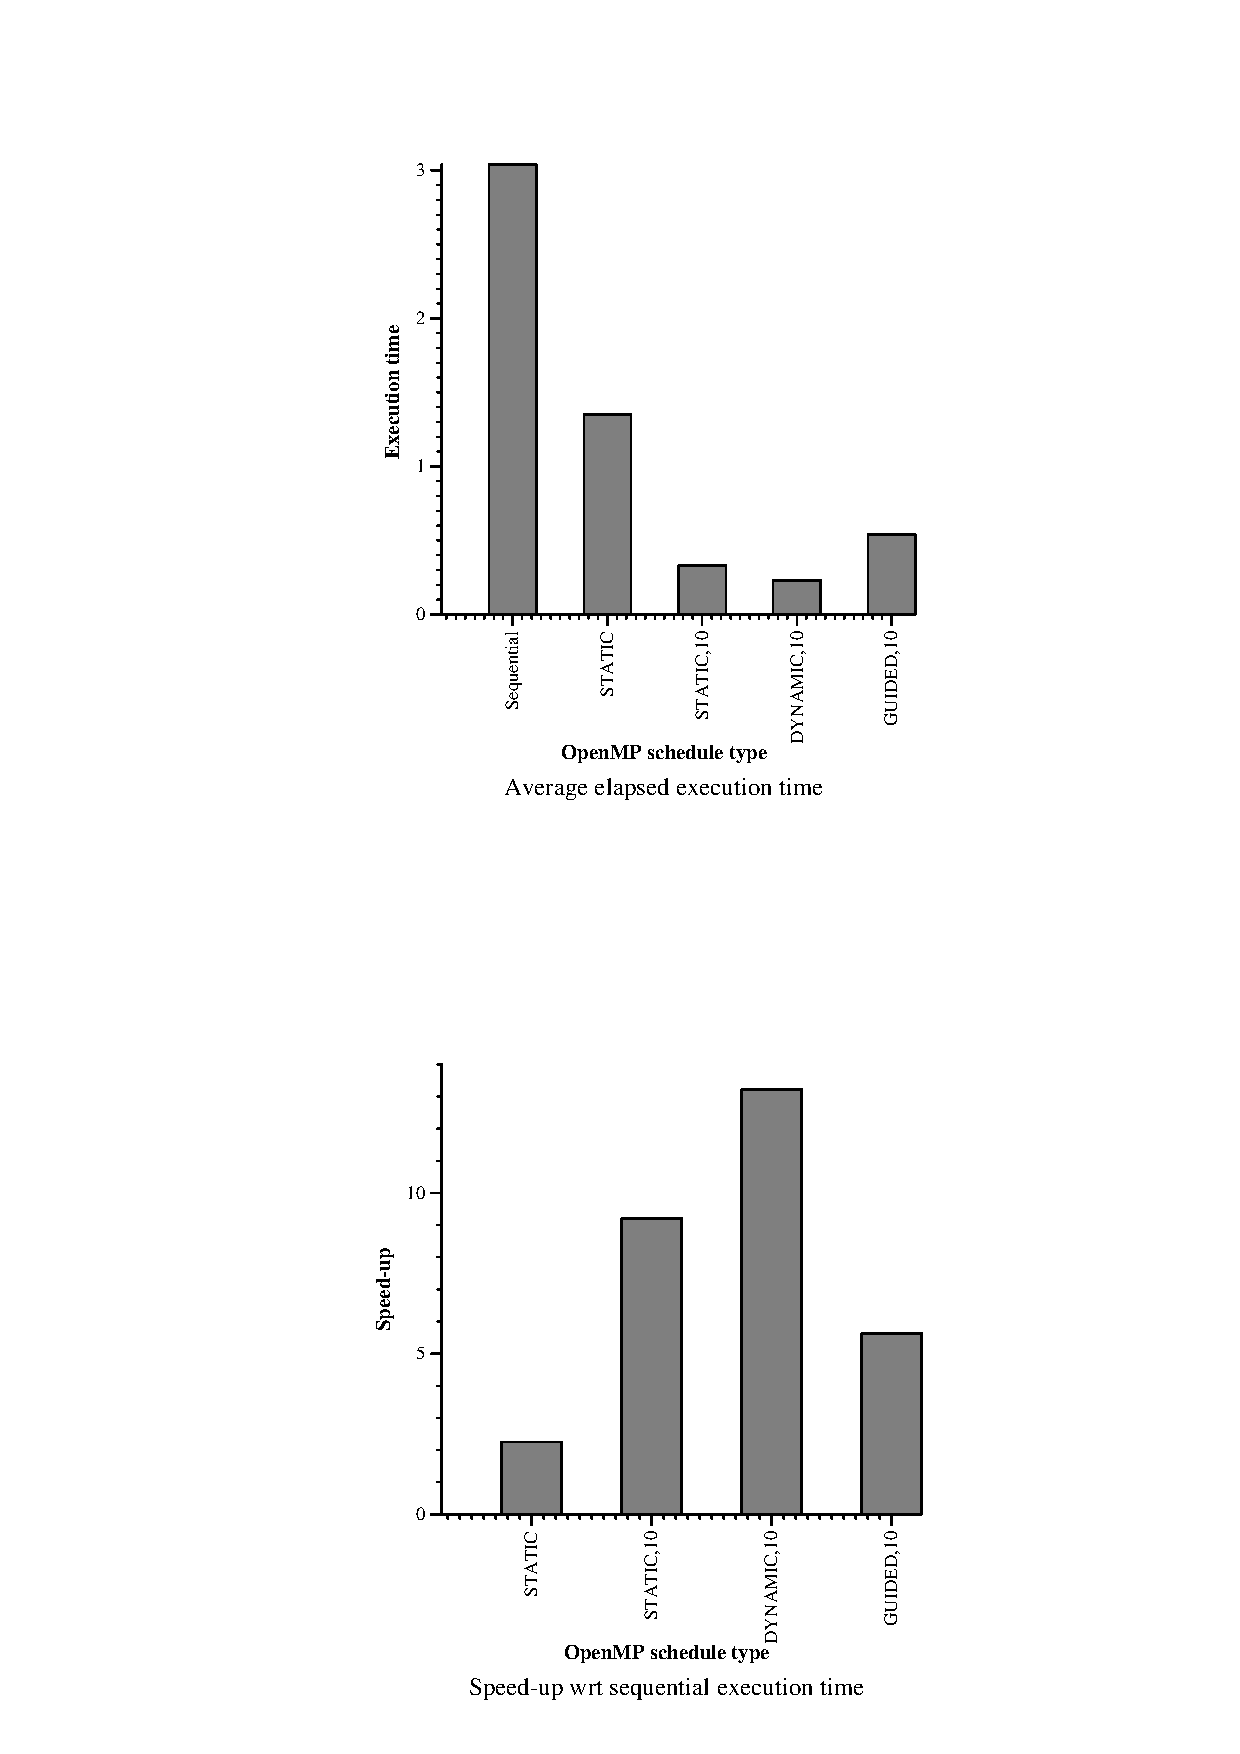
\includegraphics[trim={5cm 16cm 5cm 2cm}, clip, width=\textwidth] {images/mandel-omp-for-row-schedule.pdf}
	\end{minipage}
	\begin{minipage}[t]{0.49\textwidth}
		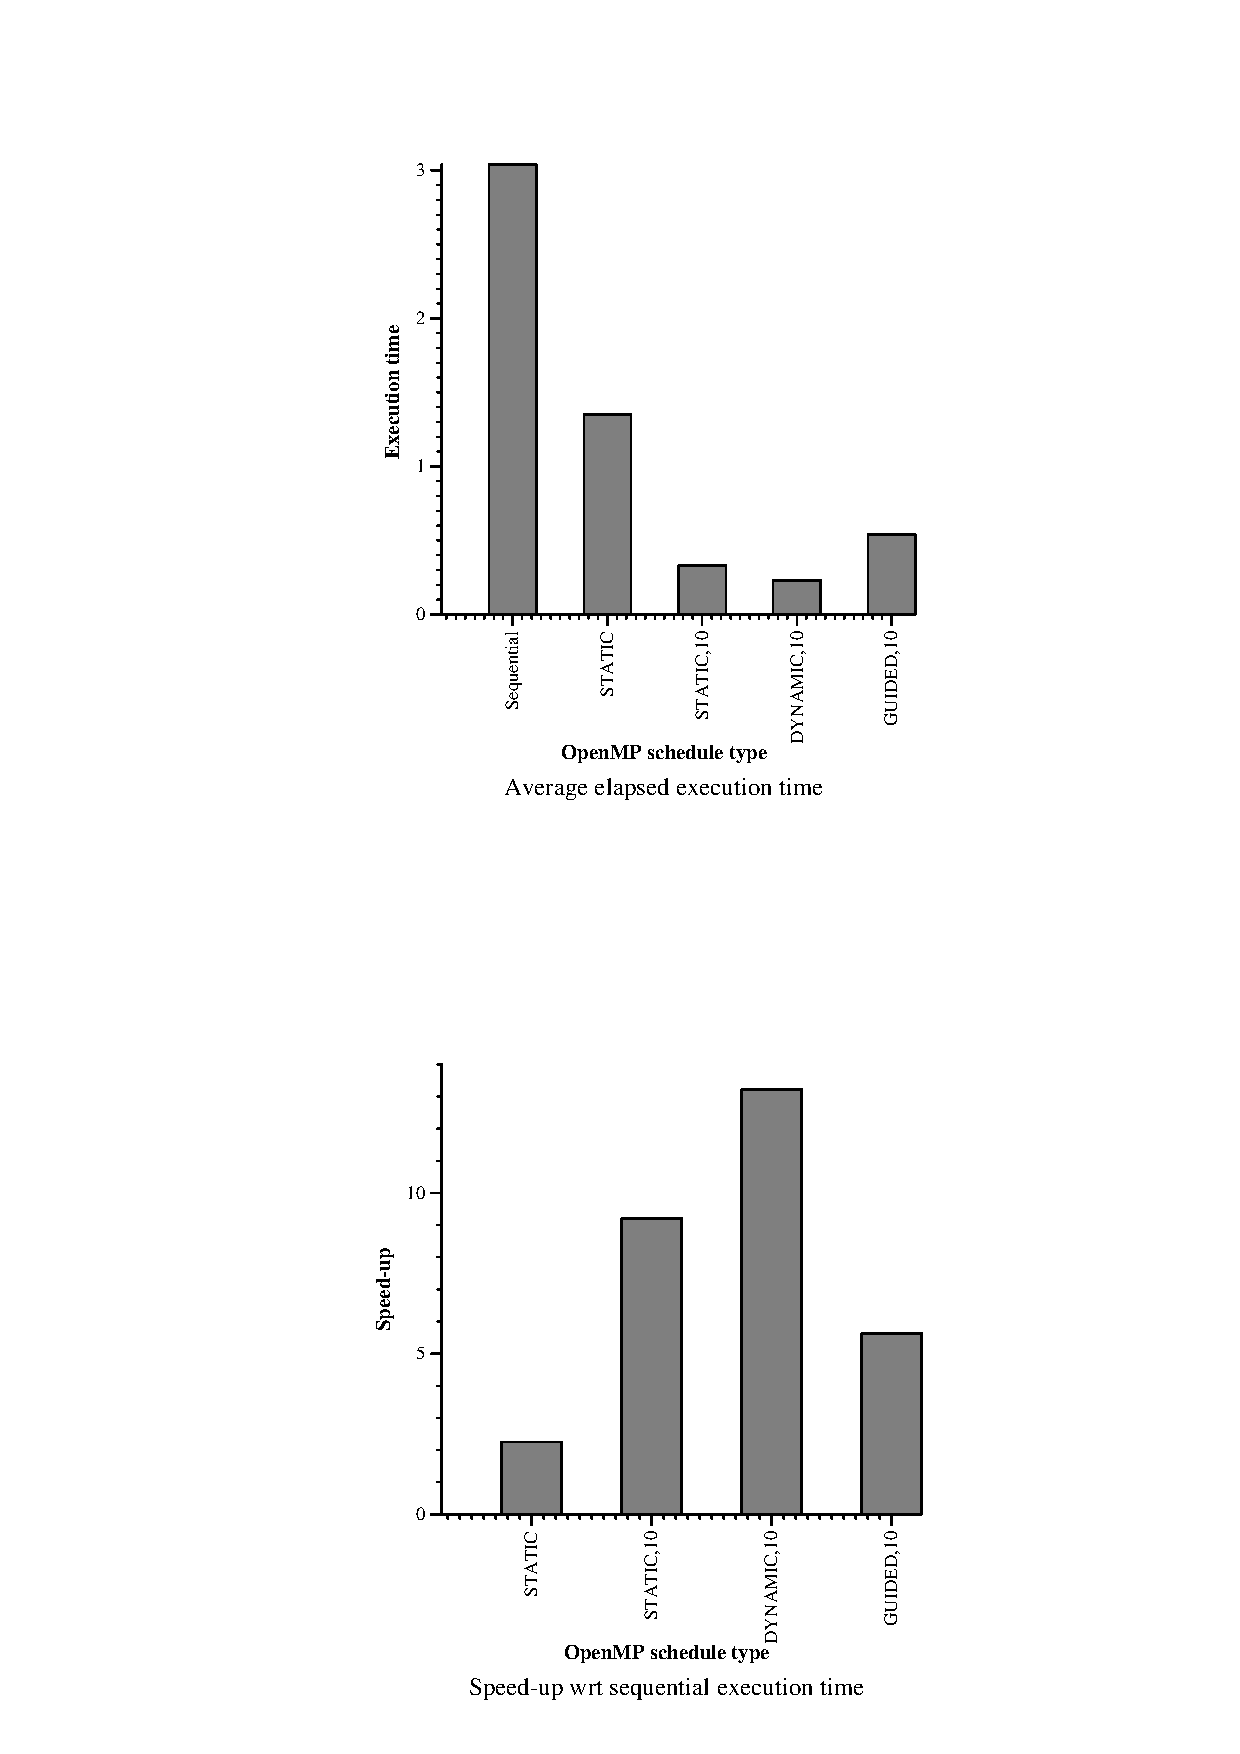
\includegraphics[trim={5cm .8cm 5cm 18cm}, clip, width=\textwidth] {images/mandel-omp-for-row-schedule.pdf}
	\end{minipage}
	\caption{Execution time and speedup for \textit{Row} decomposition}
\end{figure}

\begin{figure}[H]
	\centering
	\begin{minipage}[t]{0.49\textwidth}
		\includegraphics[trim={5cm 14cm 5cm 4.5cm}, clip, width=\textwidth] {images/mandel-omp-for-point-schedule.pdf}
	\end{minipage}
	\begin{minipage}[t]{0.49\textwidth}
		\includegraphics[trim={5cm 2.5cm 5cm 15.5cm}, clip, width=\textwidth] {images/mandel-omp-for-point-schedule.pdf}
	\end{minipage}
	\caption{Execution time and speedup for \textit{Point} decomposition}
\end{figure}

As it can be seen with \textit{Row} decomposition the obtained speedups are better than with the \textit{Point} decomposition. This is because \textit{Point} decomposition causes more schedule events that stop the threads and increasing the overhead.

\begin{enumerate}[resume]
	\item For the \textit{Row} parallelization strategy, complete the following table with the information extracted from the \textit{Extrae} instrumented executions (with 8 threads and \texttt{-i 10000}) and analysis with \textit{Paraver}, reasoning about the results that are obtained.
\end{enumerate}

\begin{table}[H]
	\centering
	\tablinesep=0.5cm
	\begin{tabular}{p{5cm}|rrrr}
		& \textbf{static} & \textbf{static, 10} 
		& \textbf{dynamic, 10} & \textbf{guided, 10} \\
		\hline
		Running average time per thread & 
		240,12 ms & 208,03 ms & 176,22 ms & 209,46 ms \\
		Execution unbalance (average time divided per maximum time) & 
		0,239 & 0,621 & 0,881 & 0,389 \\
		\texttt{SchedForkJoin} (average time per thread or time if only one does) & 
		125,64 ms & 31,22 ms & 489,64 ms & 66,66 ms
	\end{tabular}
	\caption{Table for \textit{Row} parallelization strategy}
\end{table}

It can be seen that the dynamic is the strategy with the lowest time per thread and the highest balance. This is because every time a thread finishes it requests another chunk and this causes to all the threads to do more or less the same work. However, the static strategy cannot do this because once a thread finishes all his work it remains waiting for the other threads to finish instead of helping them.

\end{document}